\section{studio qualitativo delle soluzioni}
\label{sec:studio_qualitativo_edo}

Non sempre è possibile determinare esplicitamente le soluzioni
di una equazione differenziale.
Ci proponiamo quindi di trovare dei metodi per
determinare alcune proprietà salienti delle soluzioni, senza
doverle determinare esplicitamente.
Considereremo unicamente equazioni del primo ordine in forma normale:
\begin{equation}\label{eqdiff}
	u'(x)= f(x,u(x))
\end{equation}
con $f\colon \Omega \subset \RR^2\to \RR$.

Ricordiamo che se $f$ soddisfa la condizione di Cauchy-Lipschitz
(definizione~\ref{def:cauchy_lipschitz}), in particolare
se $f$ è di classe $C^1$ allora i grafici delle soluzioni
massimali dell'equazione differenziale~\eqref{eqdiff}
\emph{fibrano} la regione $\Omega$ nel senso che per ogni punto di
$\Omega$ passa una unica soluzione massimale (teorema~\ref{th:cauchy_lipschitz}
di Cauchy-Lipschitz e proposizione~\ref{prop:separazione_soluzioni}).
Inoltre la proposizione~\ref{prop:edo_massimale} ci dice
che le soluzioni massimali escono da qualunque compatto contenuto in
$\Omega$ ovvero raggiungono sempre la frontiera di $\Omega$.

\begin{example}\label{ex:edo_4630b}
Sia $u$ la soluzione massimale del problema di Cauchy
\[
	\begin{cases}
		u' = \cos(u^2)\cdot \sin x, \\
		u(0) = 0.
	\end{cases}
\]
Mostrare che $u$
è definita su tutto $\RR$ (dunque la soluzione è globale).
Mostrare che $u$ è pari.
Mostrare che $u$ è periodica.
Mostrare che $u(x)\ge 0$ per ogni $x\in \RR$.
\end{example}
\newsavebox{\qredoquattro}\sbox{\qredoquattro}{%
\myqrshortdoclink{edo_4630b}{Studio qualitativo esempio \getrefnumber{ex:edo_4630b}}}
\begin{figure}
  \centering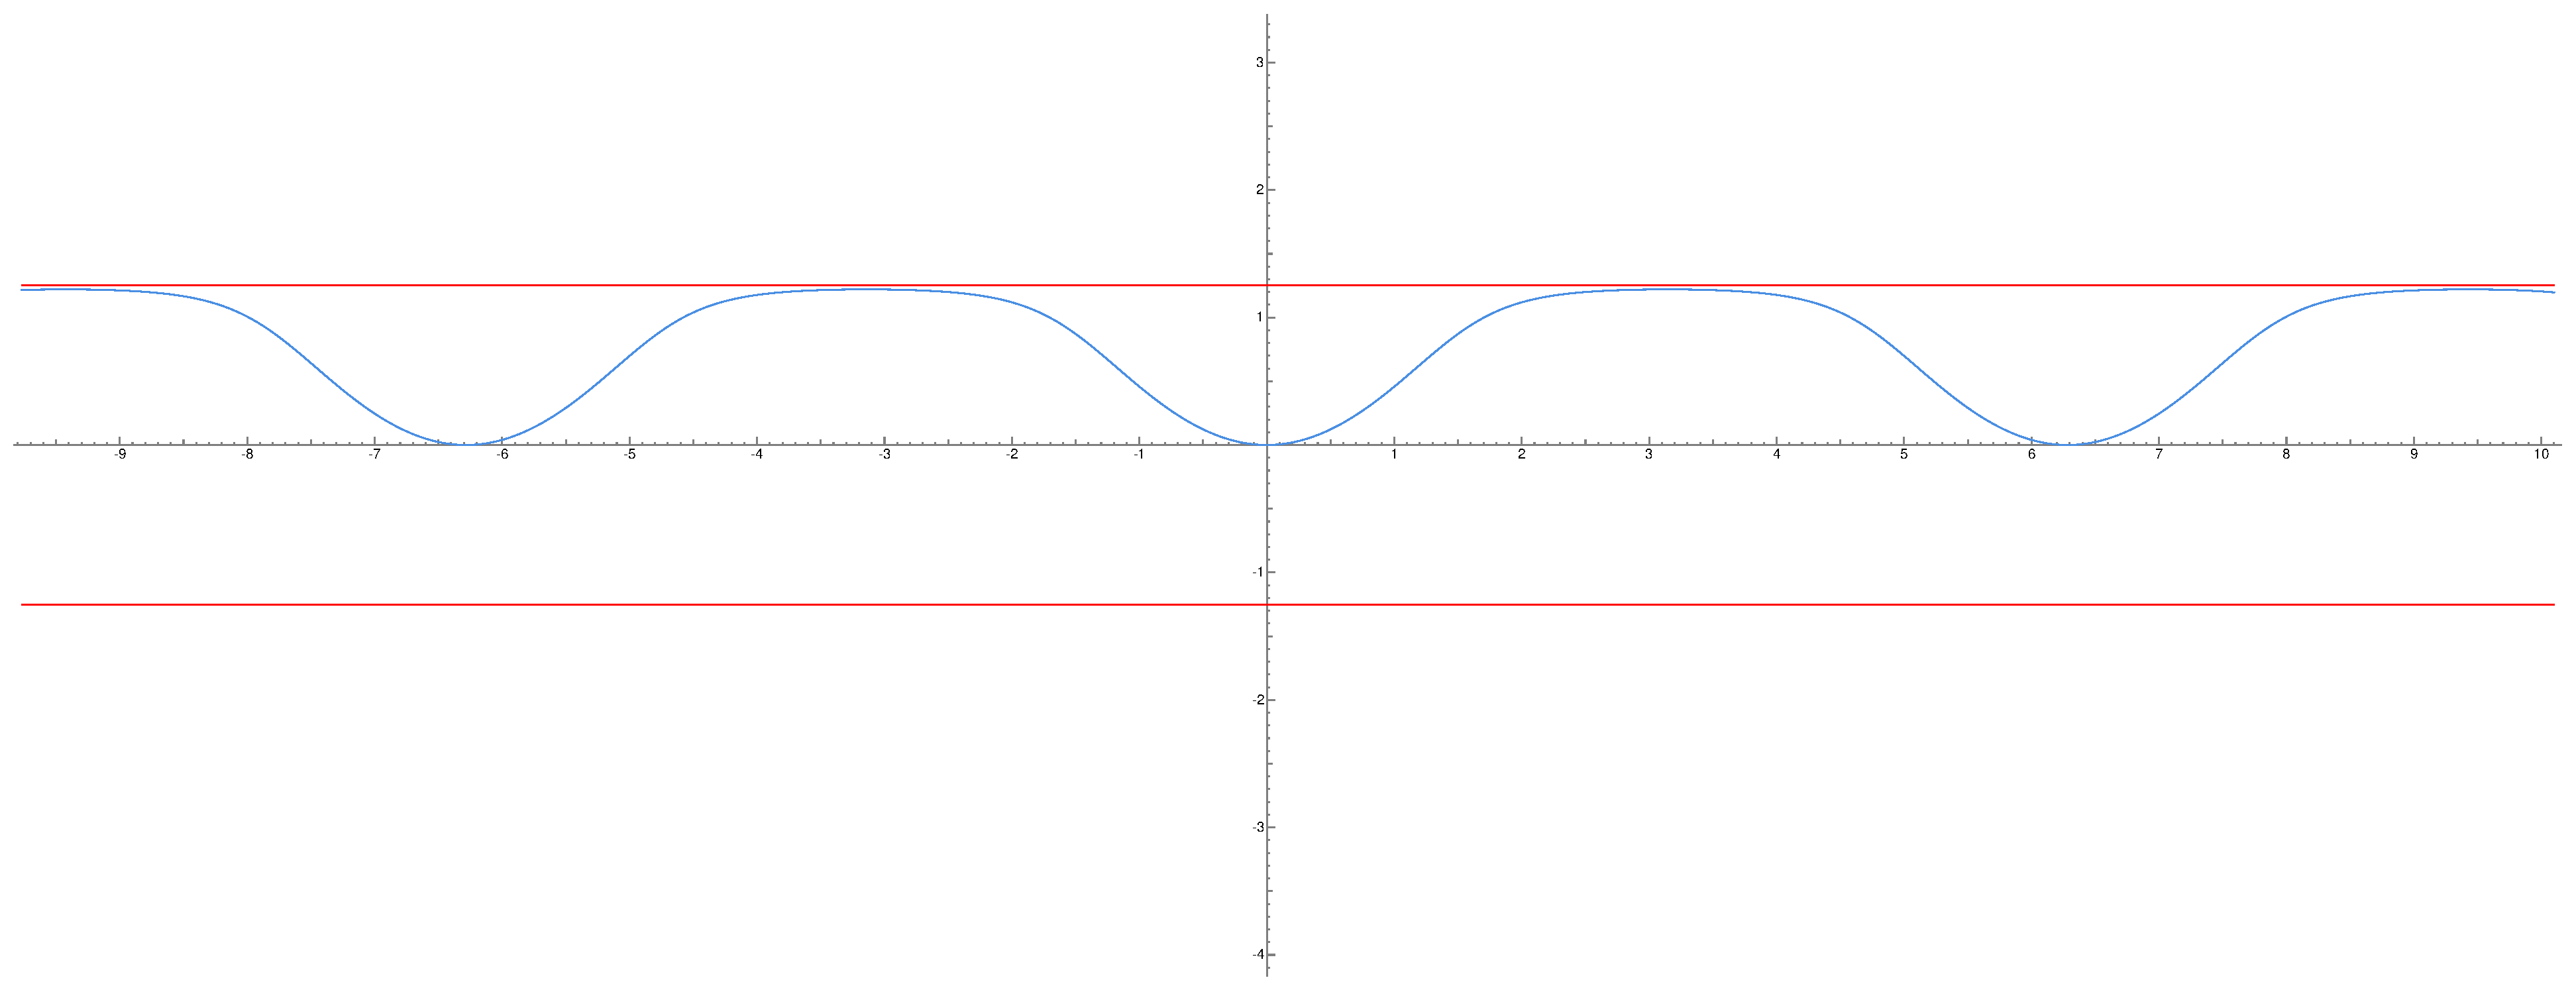
\includegraphics[width=\textwidth]{edo_4630b}
  \caption{Studio qualitativo dell'esempio~\ref{ex:edo_4630b}.
  \ifwidemargin\\\\\fi%
  \usebox{\qredoquattro}}
  \label{fig:edo_4630b}
\end{figure}
%
\begin{proof}[Svolgimento.]
In questo caso si ha $f(x,y)=\cos y^2\cdot \sin x$, che \`e una funzione
di classe $C^1$ su tutto $\Omega=\RR^2$.
Vale dunque il teorema di esistenza ed
unicità delle soluzioni.
Notiamo inoltre (per verifica diretta)
che posto $H=\sqrt{\frac \pi 2}$, le funzionie 
costanti $u_0(x)=-H$ e $u_1(x)=H$ sono
soluzioni dell'equazione differenziale (\ref{eqdiff})
in quanto $f\enclose{x,\pm H}=0$ per ogni $x\in \RR$
(soluzioni \emph{stazionarie}).
Per la proposizione~\ref{prop:separazione_soluzioni},
il grafico della soluzione $u(x)$
non può toccare i grafici delle due funzioni $u_0$ e $u_1$ e visto
che $u(0)=0$ e che $u$ è una funzione continua significa
che per ogni $x$ si ha $-H < u(x) < H$.
Consideriamo ora il compatto
$K_M=[-M,M] \times [-H,H]$.
Sappiamo che la soluzione
massimale $u(x)$ del problema di Cauchy preso in considerazione deve
uscire da ogni compatto $K_M$
(proposizione~\ref{prop:edo_massimale}).
Visto però che $u(x)\in (-H,H)$ significa che necessariamente
il grafico della soluzione massimale $u(x)$
raggiunge i due segmenti verticali
$x=-M$ e $x=M$ e dunque l'intervallo massimale di esistenza
contiene l'intervallo $[-M,M]$.
Siccome questo è vero per ogni $M$, l'intervallo massimale
di esistenza della soluzione è $I=\RR$ e dunque la soluzione
è globale.

Dimostriamo che $u$ è pari. Sia $v(x)=u(-x)$. 
Si ha 
\[ 
    v'(x) = -u'(-x) 
    = -\cos(u^2(-x))\cdot \sin(-x) 
    = \cos(v^2(x))\cdot \sin(x)
\]
da cui risulta che $v$ soddisfa la stessa equazione differenziale 
di cui $u$ è soluzione. 
Inoltre $v(0)=u(0)=0$ e quindi $u$ e $v$ sono soluzioni dello 
stesso problema di Cauchy. Per unicità della soluzione 
deve essere $u(x)=v(x)$ per ogni $x$ e quindi $u(-x)=u(x)$, come 
volevamo dimostrare.
  
Dimostriamo ora che $u$ è $2\pi$-periodica.
Sia $w(x)=u(x+2\pi)$. Si ha allora 
\[
  w'(x) = u'(x+2\pi) = \cos(u^2(x+2\pi))\cdot \sin(x+2\pi) 
  = \cos(w^2(x))\cdot \sin(x) 
\]
dunque, di nuovo, $w$ soddisfa la stessa equazione differenziale
di cui $w$ è soluzione. Si ha inoltre 
\[
  u(-2\pi) - w(-2\pi) = u(2\pi) - u(0) = w(0) - u(0).
\]
Questo significa che $u-v$ assume segno opposto nei punti 
$a=-2\pi$ e $b=0$ e quindi, per il teorema~\ref{th:valori_intermedi}
dei valori intermedi ci deve essere un punto in cui le due 
$u-v$ si annulla. In tale punto ho due soluzioni dello stesso 
problema di Cauchy e dunque, per l'unicità della soluzione, 
dobbiamo concludere che $u(x)=v(x)$ per ogni $x$.
Questo significa che $u$ è $2\pi$-periodica.

Visto che $\abs{u(x)}<H$ con $H^2=\pi 2$ si ha che $\cos(u^2(x))>0$ 
e quindi $u'(x)$ ha lo stesso segno di $\sin x$: sull'intervallo 
$[0,\pi]$ la funzione $u(x)$ è crescente e su $[\pi,2\pi]$ è decrescente.
Visto che $u$ è $2\pi$-periodica si ha che $u(2\pi)=u(0)=0$ e quindi 
$0$ è il valore minimo assunto da $u$.

Si veda la figura~\ref{fig:edo_4630b}.
\end{proof}

\subsection{monotonia e punti critici delle soluzioni}

Dopo aver determinato le zone di $\Omega$ su cui vale il teorema di
esistenza e unicit\`a, \`e utile studiare il segno di $f$. Infatti
le soluzioni $u(x)$ dell'equazione differenziale (\ref{eqdiff})
saranno strettamente crescenti dove $f>0$, strettamente decrescenti
dove $f<0$ e avranno un punto critico dove $f=0$.

Un primo caso notevole è il caso in cui $f$ si annulla su una
retta orizzontale $y=c$.
In questo caso la funzione costante $u(x)=c$ è una
soluzione dell'equazione differenziale (\ref{eqdiff}).
Inoltre
(nell'ipotesi $f\in C^1$) tale costante non può essere
attraversata dalle altre soluzioni dell'equazione differenziale.

\`E importante capire se le soluzioni dell'equazione differenziale
attraversano o no la curva $\{f=0\}$. Infatti questo ci permette di
determinare il segno della derivata $u'(x)$ e quindi di ottenere
importanti informazioni sull'andamento della soluzione $u(x)$
(monotonia, massimi e minimi relativi...).

Più in generale è interessante capire quando una soluzione di una
equazione differenziale può attraversare una determinata curva.

\begin{theorem}\label{nonpassa}
Sia $u(x)$ una soluzione dell'equazione differenziale $(\ref{eqdiff})$
definita su un intervallo $I$ e sia $v(x)$ una funzione qualunque
definita su $I$, di classe $C^1$ e tale che il suo grafico sia
interamente contenuto nel dominio $\Omega$ di definizione di $f$.
Supponiamo che in un punto fissato $x_0$ interno ad $I$ si abbia
$u(x_0)<v(x_0)$ e supponiamo inoltre che per ogni $x>x_0$ si abbia
$v'(x)>f(x,v(x))$. Allora per ogni $x>x_0$ si ha $u(x)<v(x)$.

Analogamente se $u(x_0)>v(x_0)$ e se per ogni $x$ si ha
$v'(x)<f(x,v(x))$ risulterà $u(x)>v(x)$ per ogni $x>x_0$.

Risultati analoghi si hanno per $x<x_0$.
\end{theorem}

\begin{proof}
Supponiamo per assurdo che l'insieme $J=\{x\in I: x\ge x_0\
\mathrm{e}\ u(x)=v(x)\}$ non sia vuoto.
Tale insieme è chiuso ed
inferiormente limitato, quindi se non è vuoto, ammette minimo.
Sia $\bar x$ il minimo di $J$.
Sicuramente $\bar x>x_0$ in quanto $u(\bar
x)=v(\bar x)$.
Inoltre per ogni $x\in \left[x_0,\bar x\right[$ si ha
$u(x)-v(x)<0$ e quindi $u'(\bar x) \ge v'(\bar x)$ (in quanto
il rapporto incrementale sinistro di $u-v$ è sempre positivo).

Questo è assurdo in quanto per ipotesi si ha invece $u'(\bar x) =
f(\bar x, u(\bar x)) = f(\bar x ,v(\bar x)) < v'(\bar x)$.
\end{proof}

Se ad esempio $v(x)$ è una funzione
il cui grafico è contenuto in $\{f=0\}$
(cioé $f(x,v(x))=0$) allora una soluzione $u(x)$ dell'equazione
differenziale può attraversare la curva $v(x)$ dall'alto verso il
basso nei punti in cui $v'(x)>0$ e dal basso verso l'alto nei punti
in cui $v'(x)<0$.

\newsavebox{\qrexoqt}\sbox{\qrexoqt}{%
\myqrshortdoclink{qrexoqt}{il grafico della soluzione dell'esempio \getrefnumber{ex843}}}
\begin{figure}
\centering
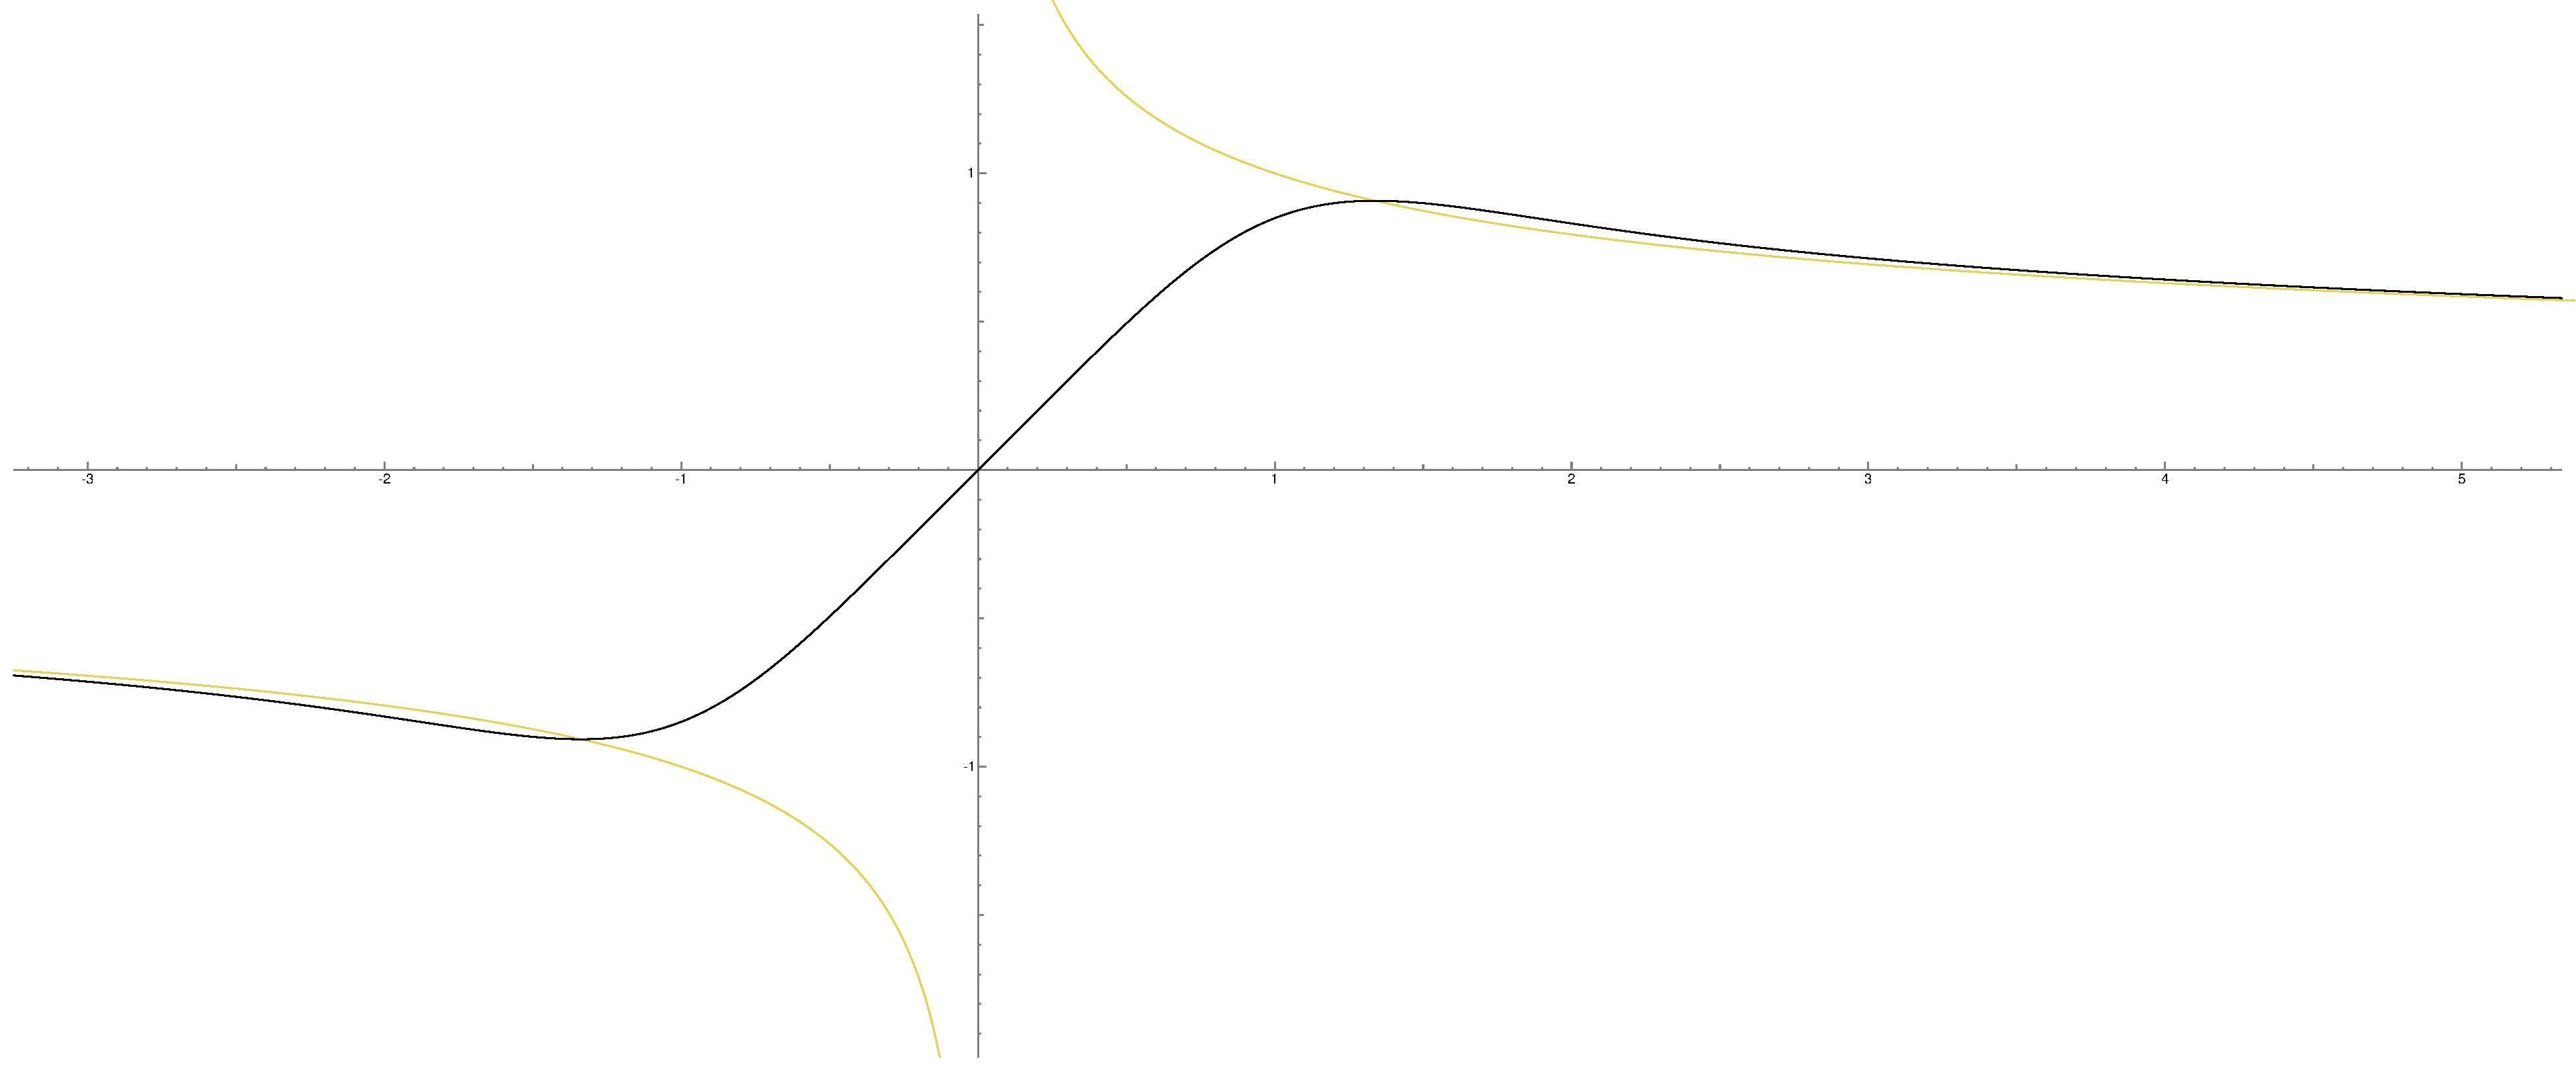
\includegraphics[width=0.8\textwidth]{ex843.pdf}
\caption{Il grafico della soluzione del problema di Cauchy nell'esempio~\ref{ex843}
\ifwidemargin\\\\\fi%
\usebox{\qrexoqt}}
\label{fig:ex843}
\end{figure}
%
\begin{example}\label{ex843}
Si consideri il seguente problema di Cauchy
\[
\begin{cases}
  u'=1-x u^3\\
  u(0)=0
\end{cases}
\]
ammette una soluzione $u(x)$ definita su tutto $\RR$.
\end{example}
%
\begin{proof}[Svolgimento.]
Posto $f(x,y)=1 - xy^3$ abbiamo che $f$ si annulla sul grafico della
funzione $u_0(x)=1/\sqrt[3] x$. Per $x>0$ la soluzione è crescente
quando si trova al di sotto della funzione $u_0$ ed è decrescente
quando si trova al di sopra. Inoltre essendo $u_0'<0$ le soluzioni possono
attraversare la funzione $u_0(x)$ solo passando da sotto a
sopra.

Sia $u(x)$ la soluzione del problema di Cauchy in questione, definita su
un intervallo massimale $I$. Il dato
iniziale è $(0,0)\in \{f>0\}$. Dunque la soluzione risulta essere
strettamente crescente in un intorno di $0$.

Vogliamo dimostrare innanzitutto che necessariamente la soluzione
incontra entrambi i rami del grafico di $u_0(x)$. Sia infatti
$\eps>0$ sufficientemente piccolo da appartenere all'intervallo
$I$ di
esistenza della soluzione e sia $\delta=u(\eps)$.
Consideriamo il compatto $K=\{(x,y):
\eps/2 \le x \le 1/\delta^2,\ 0\le y\le 1/\sqrt[3]{x}\}$. Il punto
$(\eps,u(\eps))$ è interno al compatto $K$ ma la soluzione deve
uscire dal compatto
per un qualche $x>\eps$.
La soluzione però non può toccare la
retta $y=0$ in quanto all'interno del compatto rimane sempre positiva
e crescente.
Non può neanche toccare il segmento verticale
$x=1/\delta^2$, $y\in[0,\delta]$ in quanto $u(\eps)=\delta$ e per
$x>0$ la soluzione è strettamente crescente.
Dunque necessariamente
la soluzione deve incontrare il grafico della funzione
$u_0(x)=1/\sqrt[3]{x}$ in un punto $\bar x>0$.

Nel punto $x=\bar x$ la soluzione $u(x)$ attraversa la curva
$u_0(x)$. Infatti in tale punto $u'(\bar x)=0$ mentre $u_0'(\bar
x)<0$.
Dunque in un intorno destro di $\bar x$ la soluzione si trova
al di sopra della curva $u_0(x)$ e quindi risulta essere decrescente
(in $\bar x$ la soluzione presenta un massimo relativo).

Il Teorema~\ref{nonpassa} garantisce inoltre che la soluzione non
può più riattraversare il grafico della funzione $u_0$ in quanto
$u'_0<0$. Dunque la soluzione è decrescente e limitata.
Dunque (usando come al solito la proposizione~\ref{prop:edo_massimale})
possiamo dedurre che la soluzione massimale è definita per ogni $x>0$.

Un ragionamento analogo si fa per $x<0$ ottenendo l'esistenza globale
della soluzione.
\end{proof}

\begin{example}
Dimostriamo che il problema di Cauchy
\[
\begin{cases}
	u' = -x(u^3 - \sin x) \\
	u(0) = 0
\end{cases}
\]
ammette una soluzione $u(x)$ definita su tutto $\RR$.
\end{example}
%
\begin{proof}
Sia $u(x)$ la soluzione massimale del problema di Cauchy
definita su un intervallo massimale $I$.

Mostriamo innanzitutto che $\vert u(x) \vert < 2$ per ogni $x\in
I$.
Infatti per $x>0$ sulla curva $u_1(x)=2$ si ha $f(x,2) = -x
(8-\sin x) < -x < 0 = u_1'(x)$.
Dunque per il Teorema~\ref{nonpassa} la
soluzione per $x>0$ non può mai attraversare la retta
$y=2$.
Discorso analogo si fa per la retta $y=-2$ e anche per $x<0$
mostrando che il grafico della  soluzione non può mai toccare le
rette $y=2$ e $y=-2$ né per $x>0$ né per $x<0$
e che quindi $u(x)$ risulta limitata (in realtà si
può essere più precisi e mostrare che $\vert u(x)\vert \le 1$).

A questo punto si applica, come al solito, il Teorema~\ref{prop:edo_massimale} ai
compatti $K_M=[-M,M]\times[-2,2]$ mostrando che la soluzione deve
avere esistenza globale.
\end{proof}

\subsection{teoremi di confronto}

\begin{theorem}
Sia $I\subset \RR$ un intervallo su cui sono definite due funzioni derivabili
$f(x)$ e $g(x)$.
Siano $x_1<x_2$ due punti di $I$. Se $f(x_1)<g(x_1)$ e $f(x_2)>g(x_2)$
allora esiste un punto $\bar x \in (x_1,x_2)$ tale che $f(\bar
x)=g(\bar x)$ e $f'(\bar x)\ge g'(\bar x)$.
\end{theorem}

\begin{theorem}
Consideriamo due funzioni $u(x)$ e $v(x)$ soluzioni dei rispettivi
problemi di Cauchy
\[
\begin{cases}
  u'(x)  = f(x,u(x))\\
  u(x_0) = u_0
\end{cases}
\qquad
\begin{cases}
  v'(x) = g(x,v(x))\\
  v(x_0) = v_0
\end{cases}
\]
su un intervallo $I$ che contiene il punto $x_0$.
Sia $\Omega\subset \RR^2$ un sottoinsieme degli insiemi di definizione
di $f$ e $g$ tale che i grafici delle soluzioni $u(x)$ e $v(x)$ siano
contenuti in $\Omega$ al variare di $x\in I$.
Supponiamo che per ogni $(x,y)\in\Omega$ si abbia $f(x,y)<g(x,y)$.
Allora per ogni $x\in I$, $x> x_0$ si ha $u(x)< v(x)$ mentre per ogni
$x\in I$, $x<x_0$ si ha $u(x)>v(x)$.
\end{theorem}

\begin{theorem}
Sia $f\colon (x_0,+\infty)\to \RR$ una funzione di classe
$C^1$ tale
che il limite
\[
  \lim_{x\to +\infty} f'(x) = \ell
\]
esiste, finito o infinito. Se $\ell\neq 0$ allora $f$ non può avere
un asintoto orizzontale per $x\to +\infty$.
\end{theorem}
